\section{Conclusions\label{sec:conclusions}}

Measurements of inclusive $W$ and $Z$ cross sections have been
performed using approximately 36~pb$^{-1}$ of data taken with the 
CMS detector at the LHC. 
%Individual cross section measurements
%and ratios of cross sections are precise at the level of about~3\%.
Summaries of the measurements are given 
in Figs.~\ref{fig:WZ_LEPstylePlots} and~\ref{fig:WPM_LEPstylePlots},
illustrating the good agreement of our measurements with theoretical
predictions computed at the NNLO QCD level with recent NLO PDF sets,
as well as the consistency in the measurements in the electron
and muon channels.  The ratios of our measurements to the theoretical
predictions are listed in Table~\ref{tab:RatioCMSTHY}
and pictured on Fig.~\ref{fig:RatioCMSTHY}.  

The results are in agreement with previous measurements
by ATLAS~\cite{WZATLAS:2010} and
CMS~\cite{WZCMS:2010} performed with a smaller integrated luminosity.
%The agreement is very good, with a tendency for all cross sections to be about~5\%
%lower than the theoretical prediction.  This agreement is
%better than the nominal uncertainty on the luminosity,
%indicating that the concept of using inclusive~$W$ and~$Z$ boson 
%cross sections to determine the luminosity has merit.
%
%\par
%Aside from the luminosity uncertainty which cancels 
%in the ratios, the experimental systematic uncertainties start to
%dominate the measurements reported in this Note.
%However, since  the bulk of the systematic uncertainties is of
%statistical nature,  these are expected to decrease with larger data
%samples, along with improved understanding of the CMS detector.
%

\par
Fig.~\ref{fig:WZsigmas} shows the CMS measurements together 
with measurements at lower-energy hadron colliders.
The predicted increase of the cross sections with energy is confirmed
by our measurements.

\begin{figure}
\begin{center}
  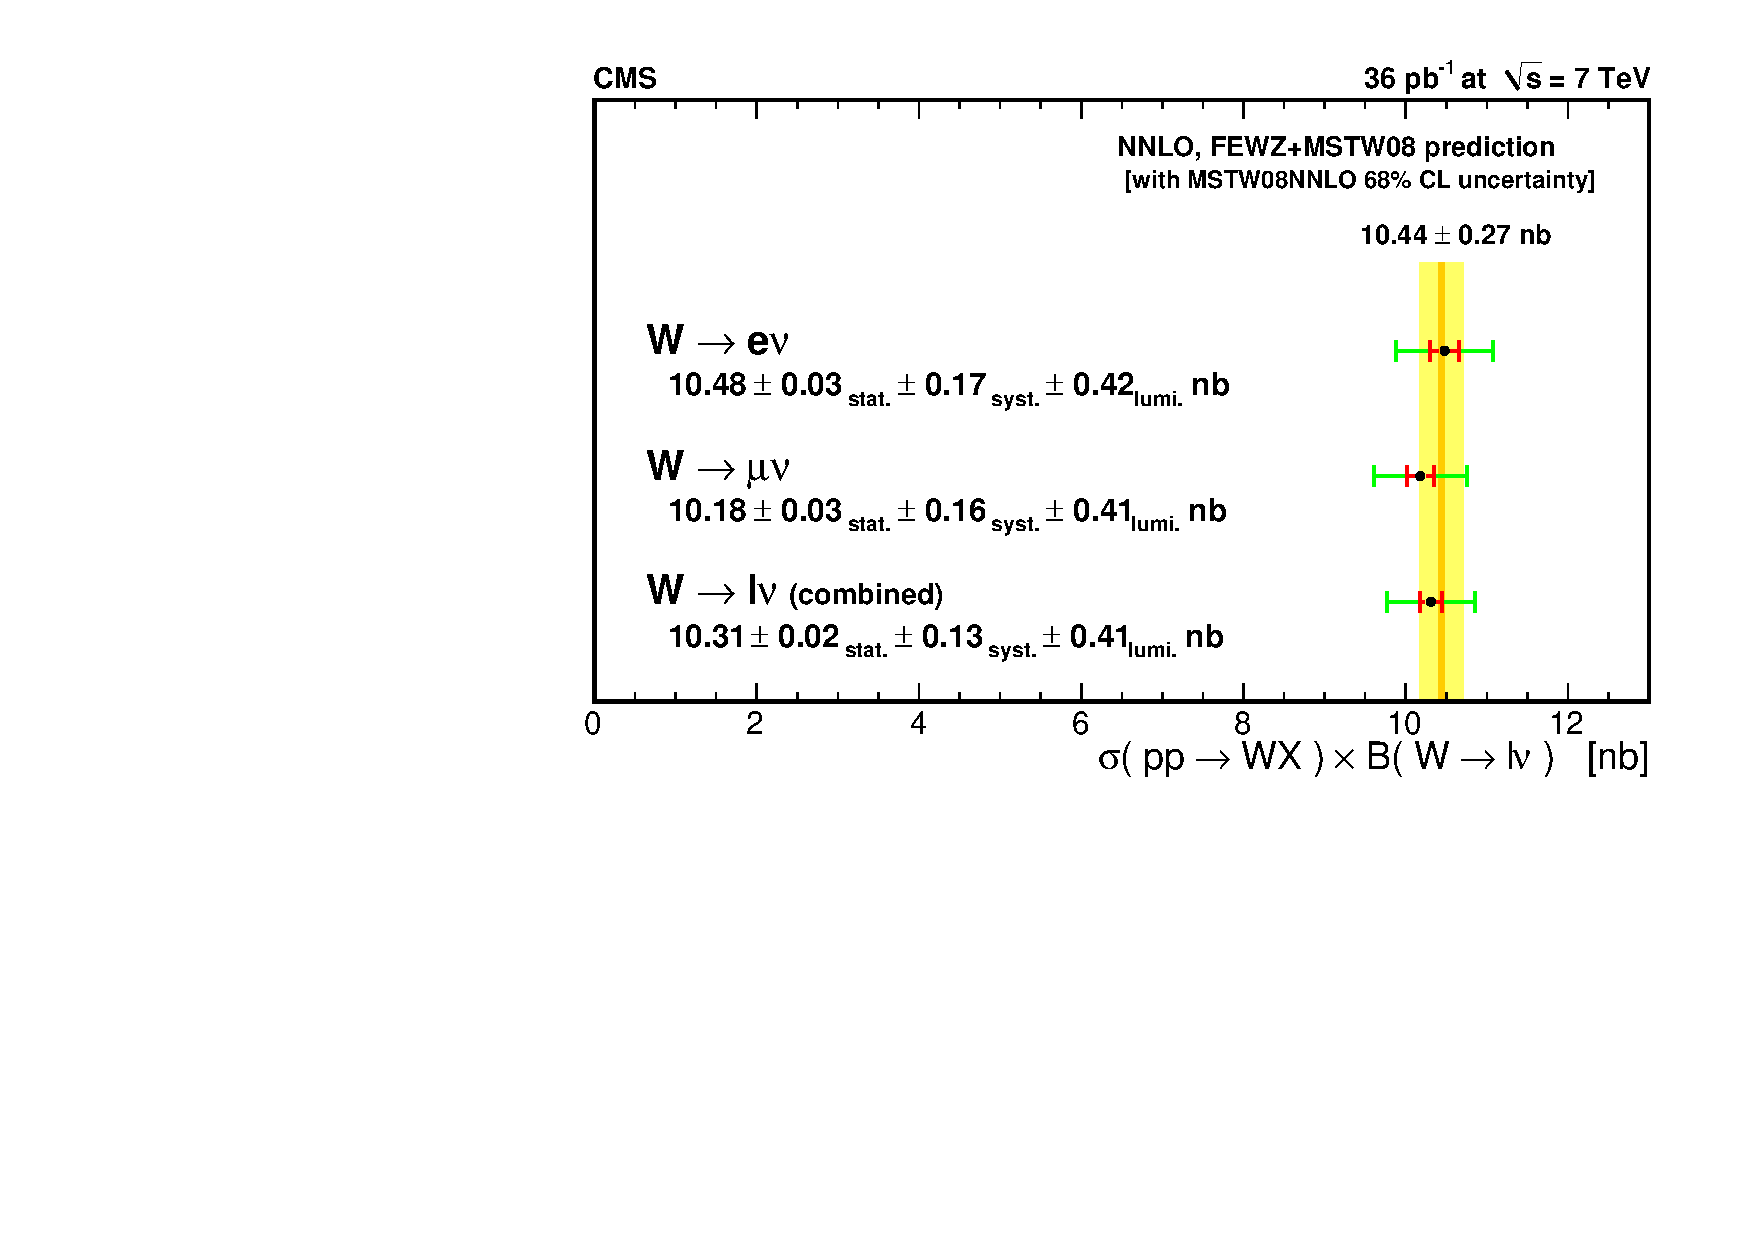
\includegraphics[width=0.49\textwidth]{figs/Results_W.pdf}
  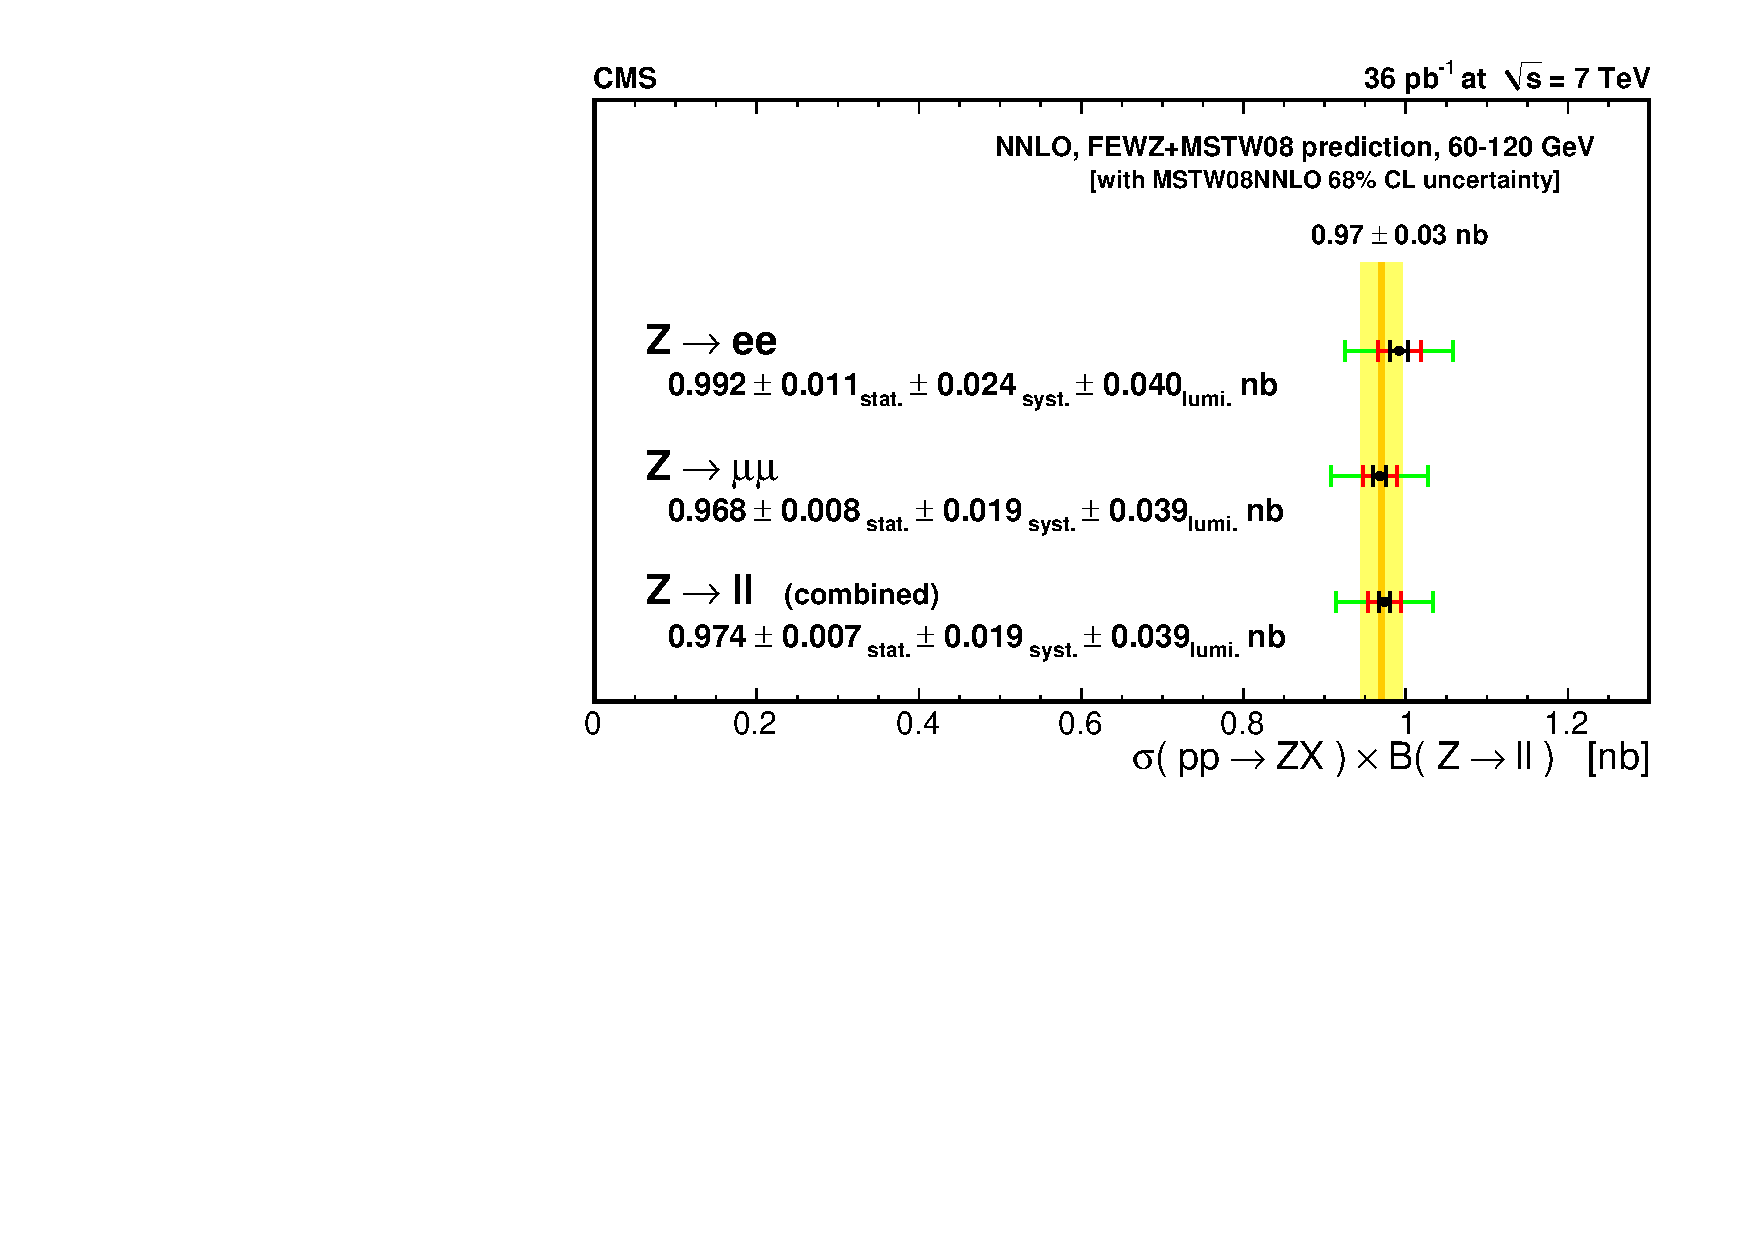
\includegraphics[width=0.49\textwidth]{figs/Results_Z.pdf}
  \\
  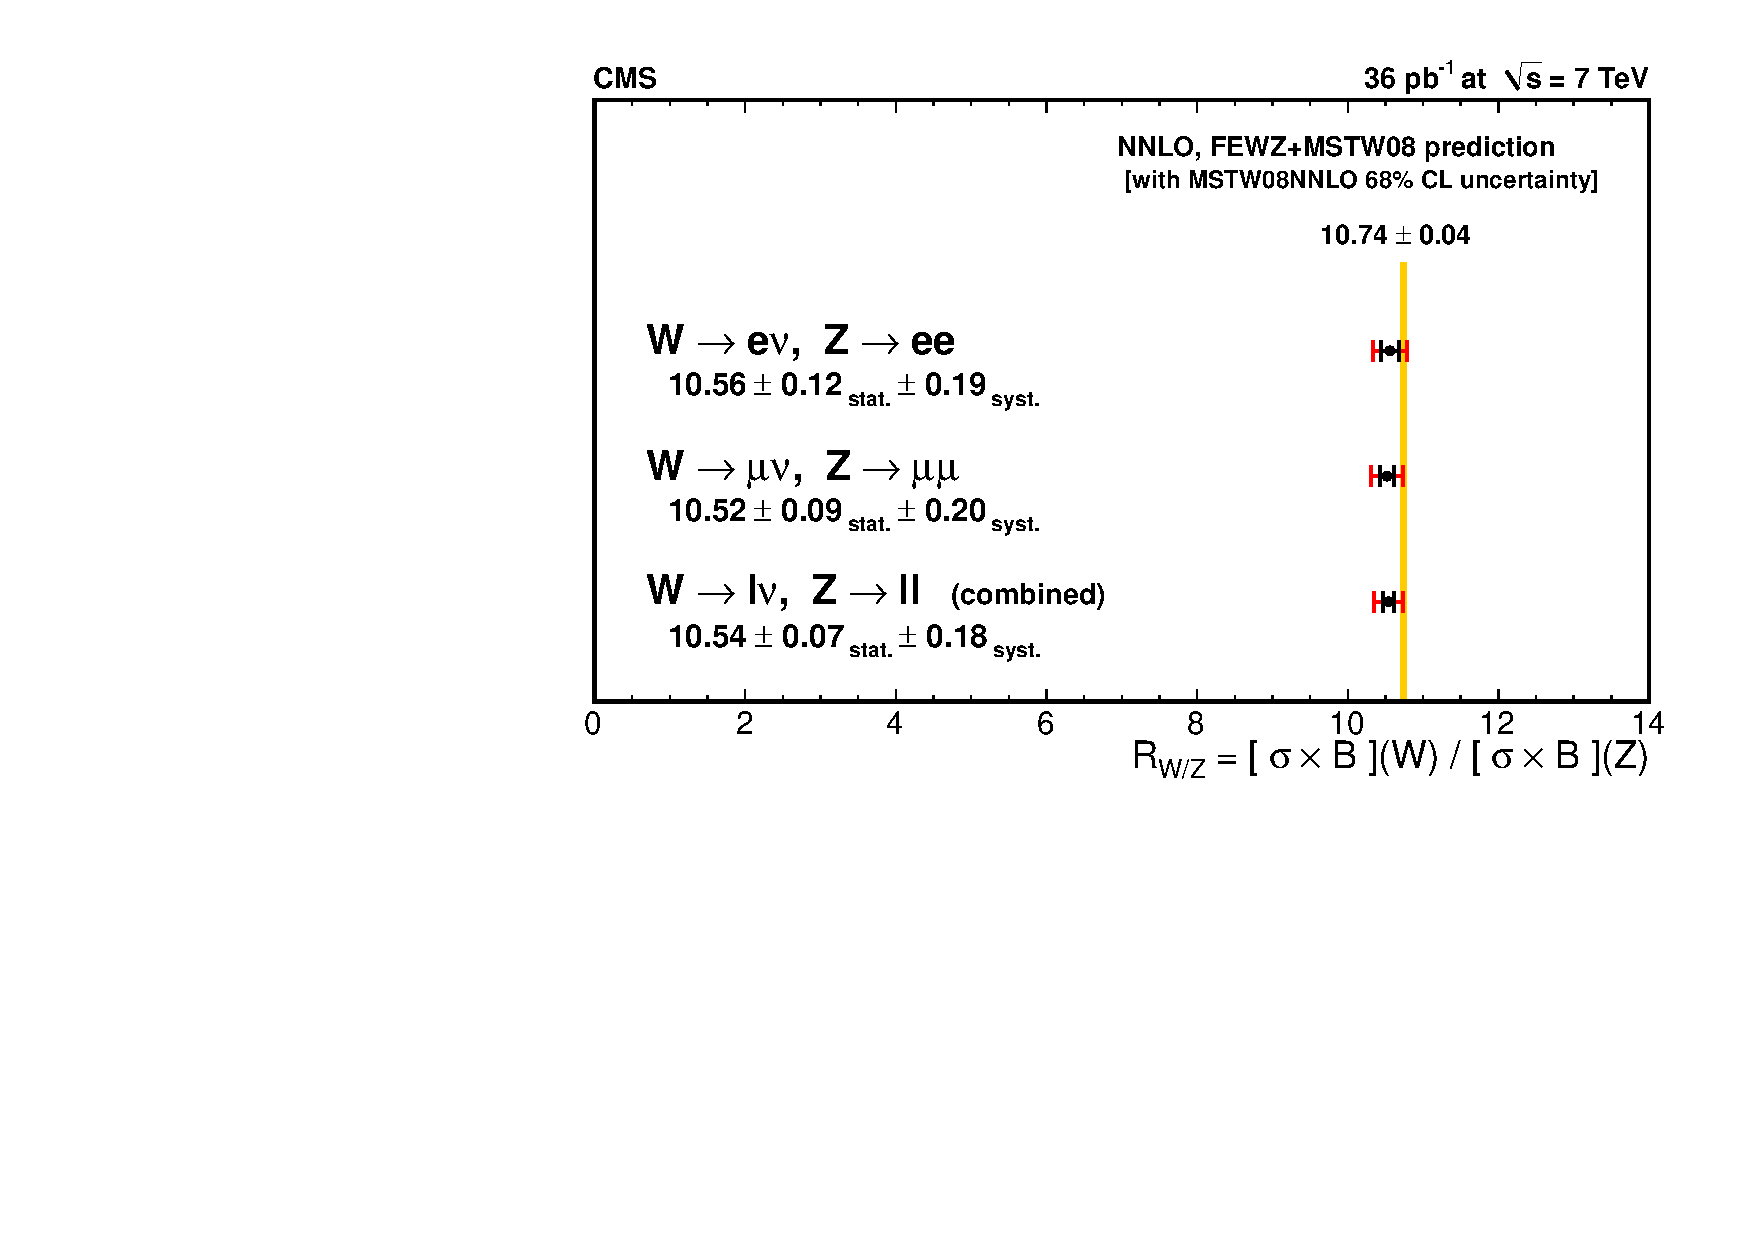
\includegraphics[width=0.49\textwidth]{figs/Results_R_WZ.pdf}
\caption[.]{\label{fig:WZ_LEPstylePlots}
Summary of results for $\Wo$ and $\Zo$ production, and ratio. }
\end{center}
\end{figure}

\begin{figure}
\begin{center}
  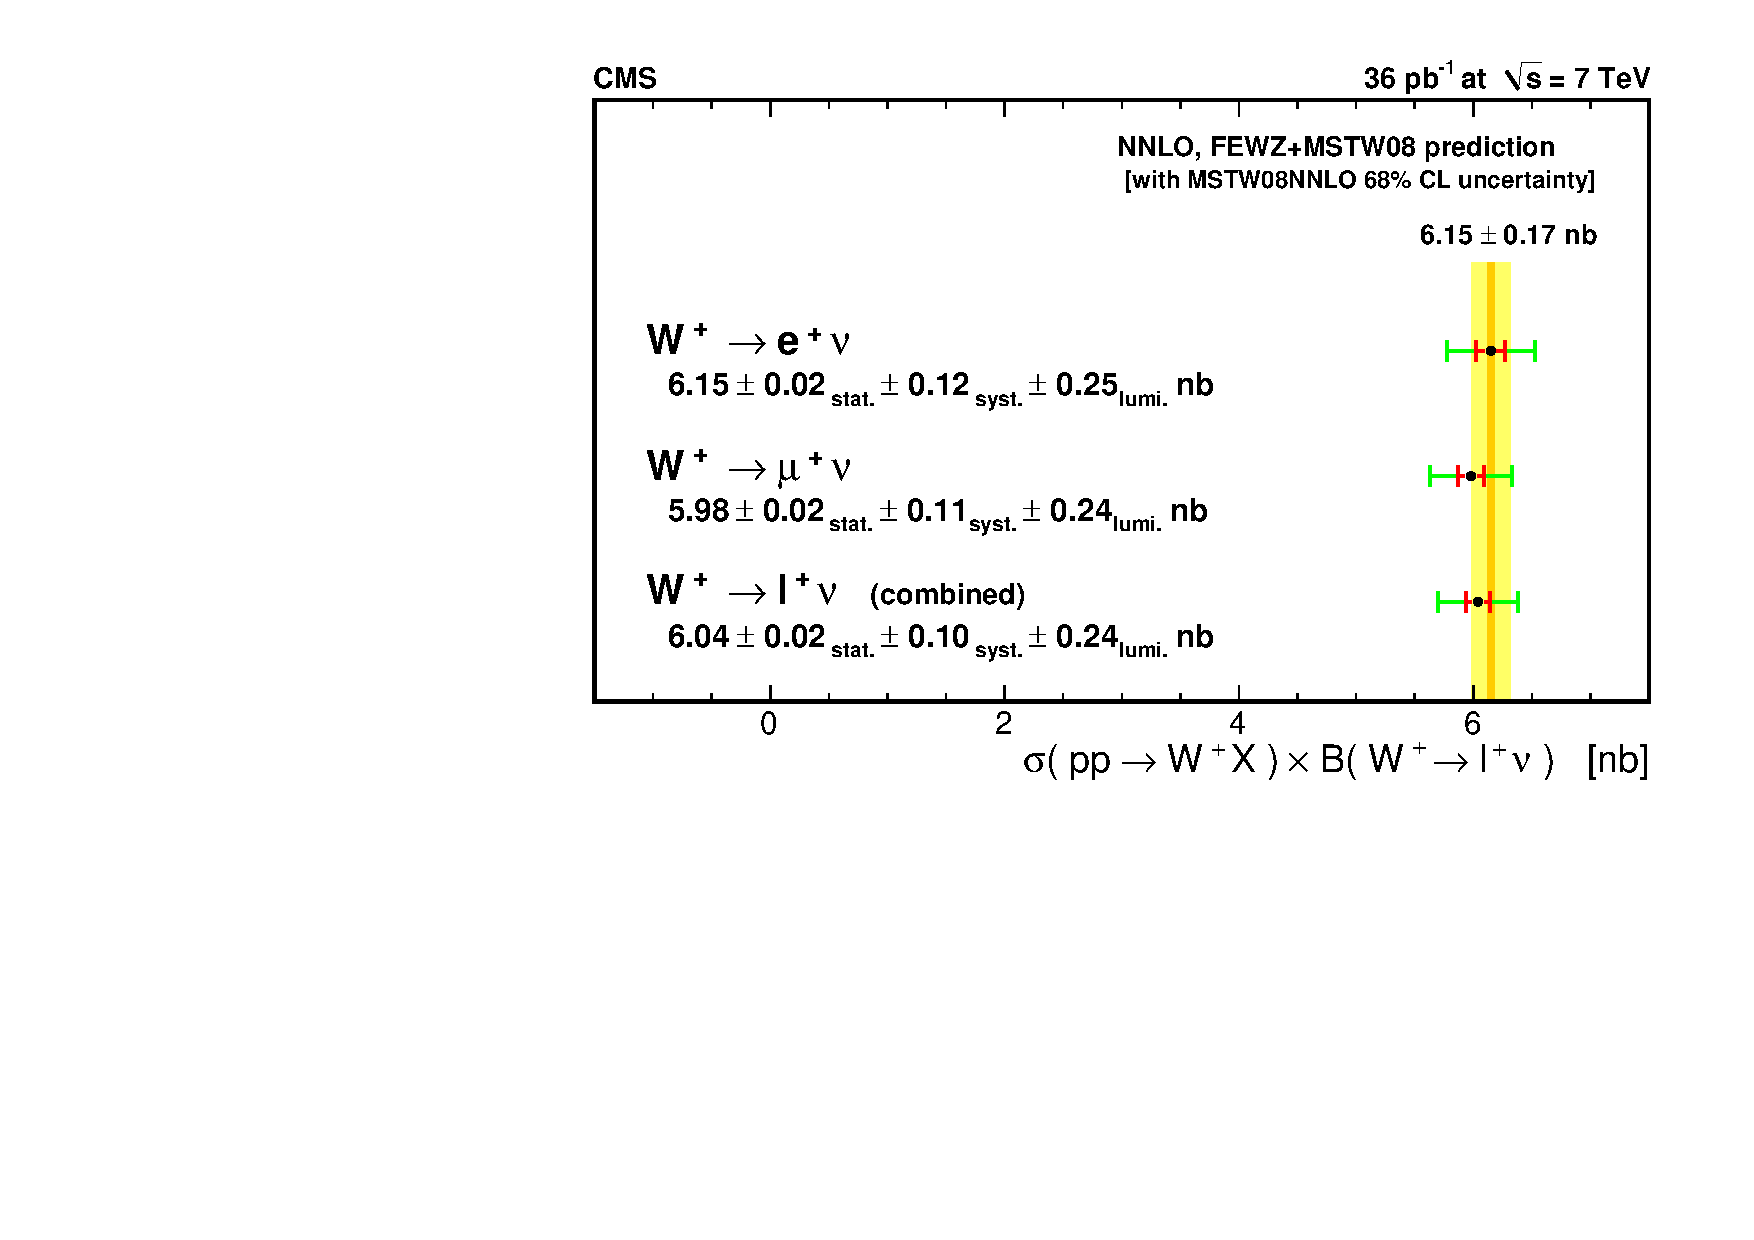
\includegraphics[width=0.49\textwidth]{figs/Results_W_plus.pdf}
  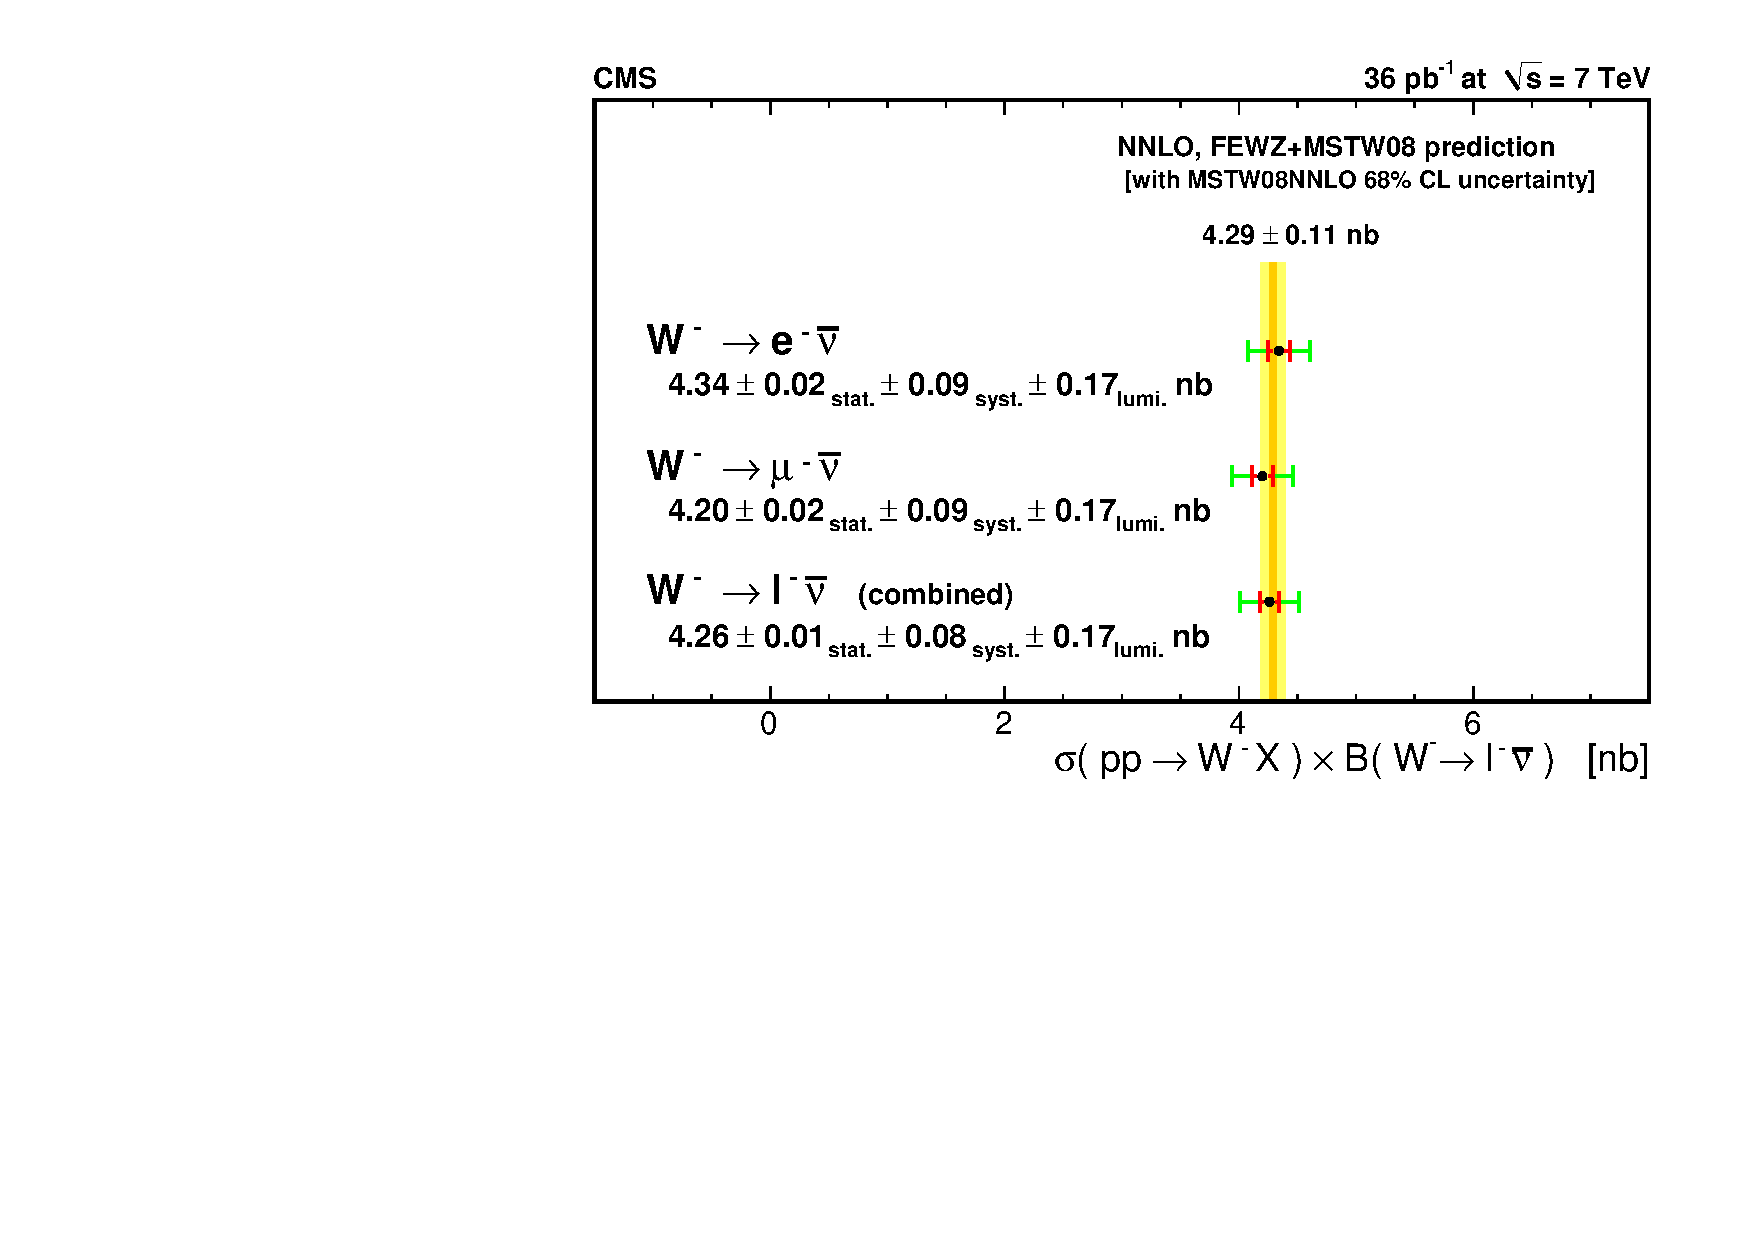
\includegraphics[width=0.49\textwidth]{figs/Results_W_minus.pdf}
\\
  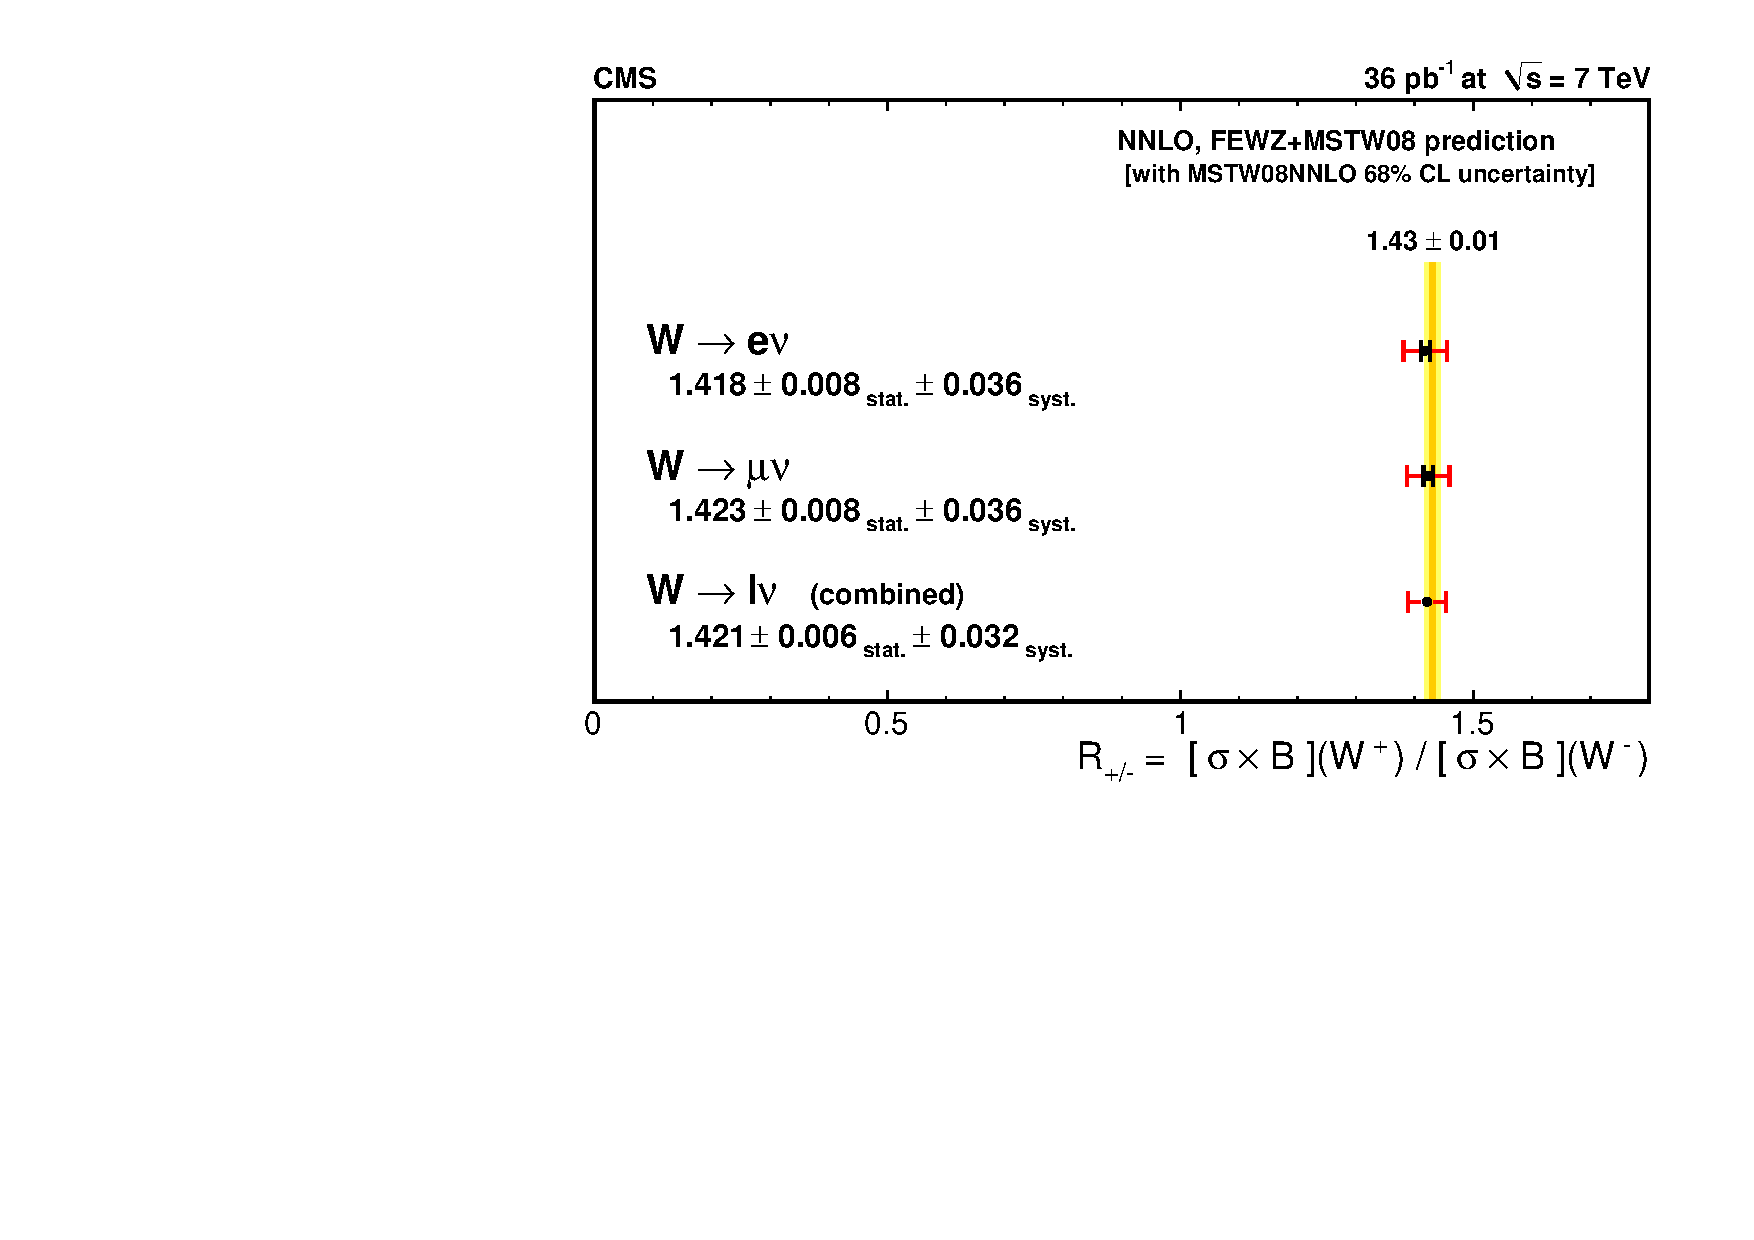
\includegraphics[width=0.49\textwidth]{figs/Results_R_WpWm.pdf}
\caption[.]{\label{fig:WPM_LEPstylePlots}
Summary of results for $\Wp$ and $\Wm$ production, and ratio. }
\end{center}
\end{figure}

% \begin{figure}
% \begin{center}
%   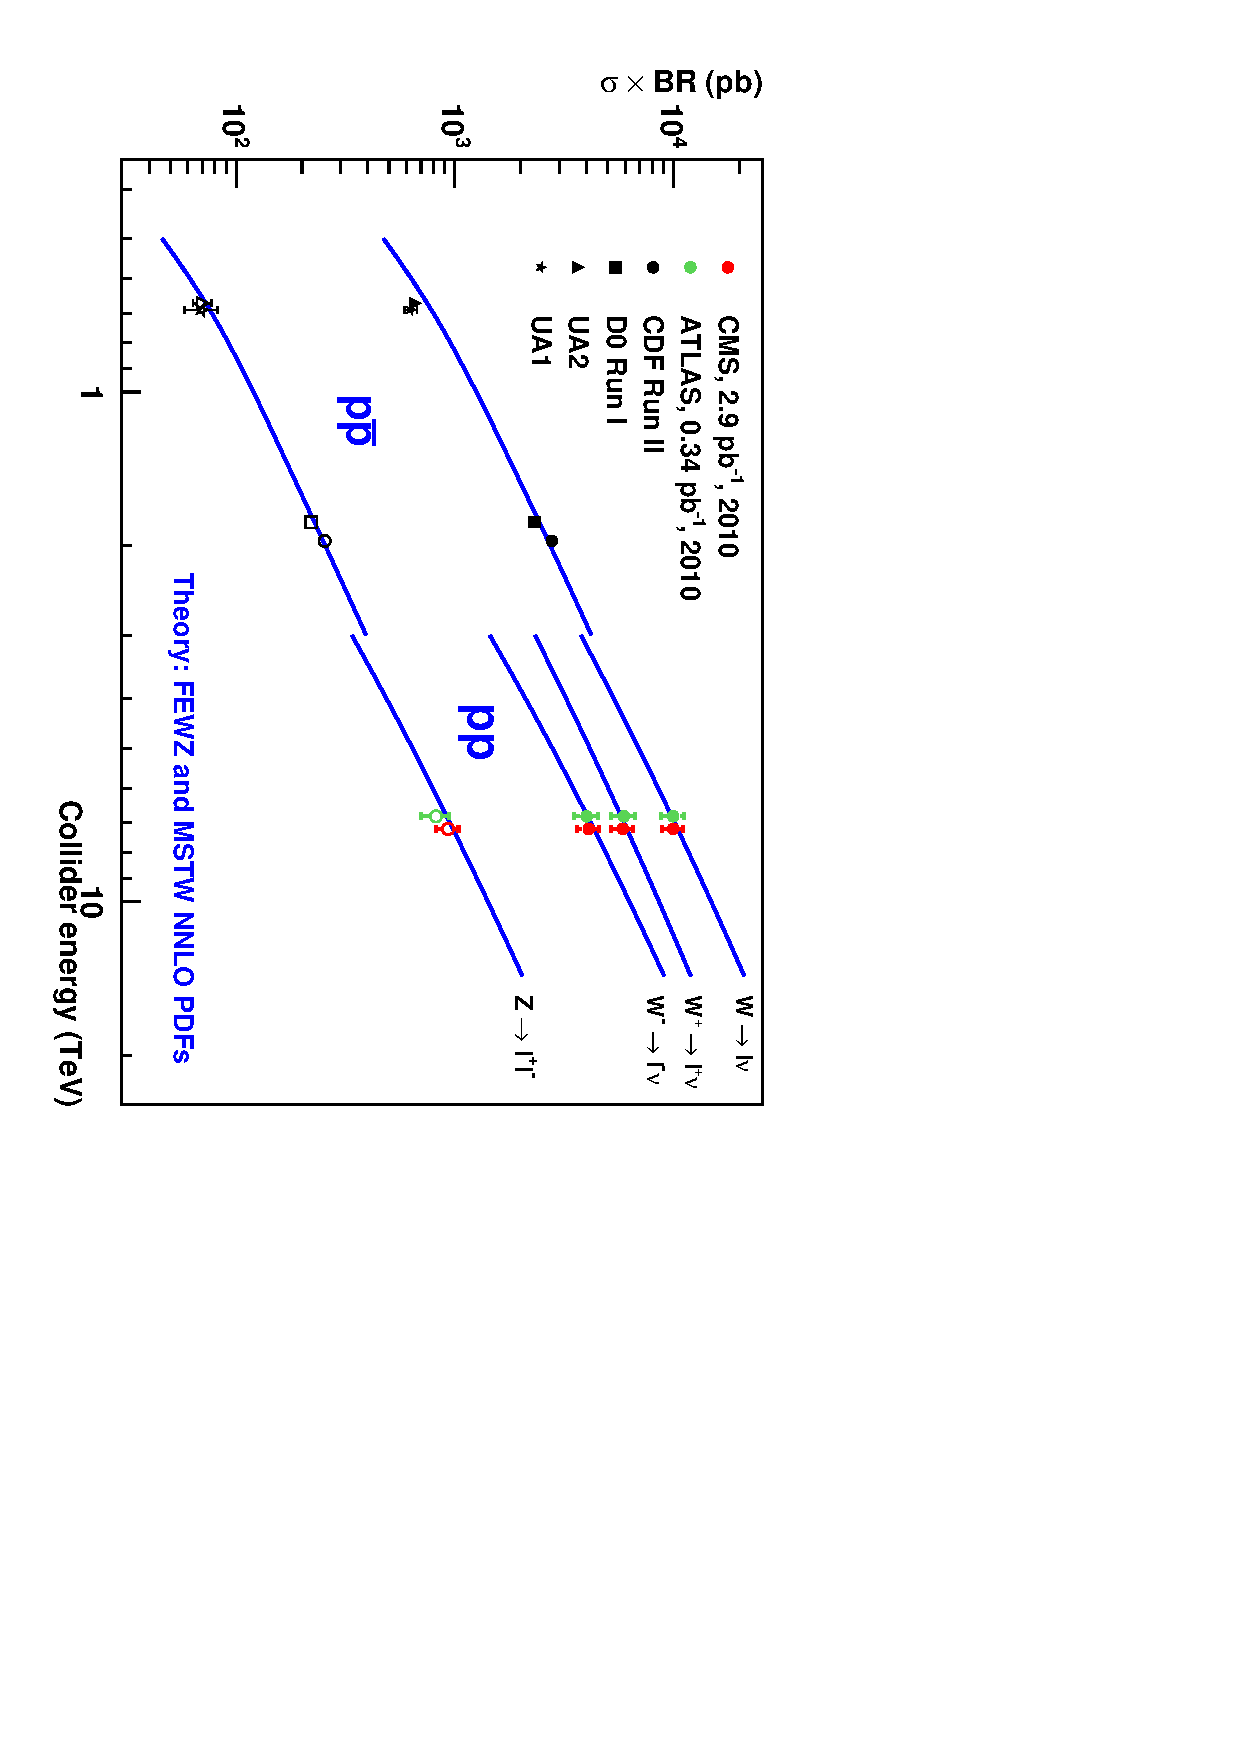
\includegraphics[width=0.49\textwidth]{figs/Results_fake.pdf}
%   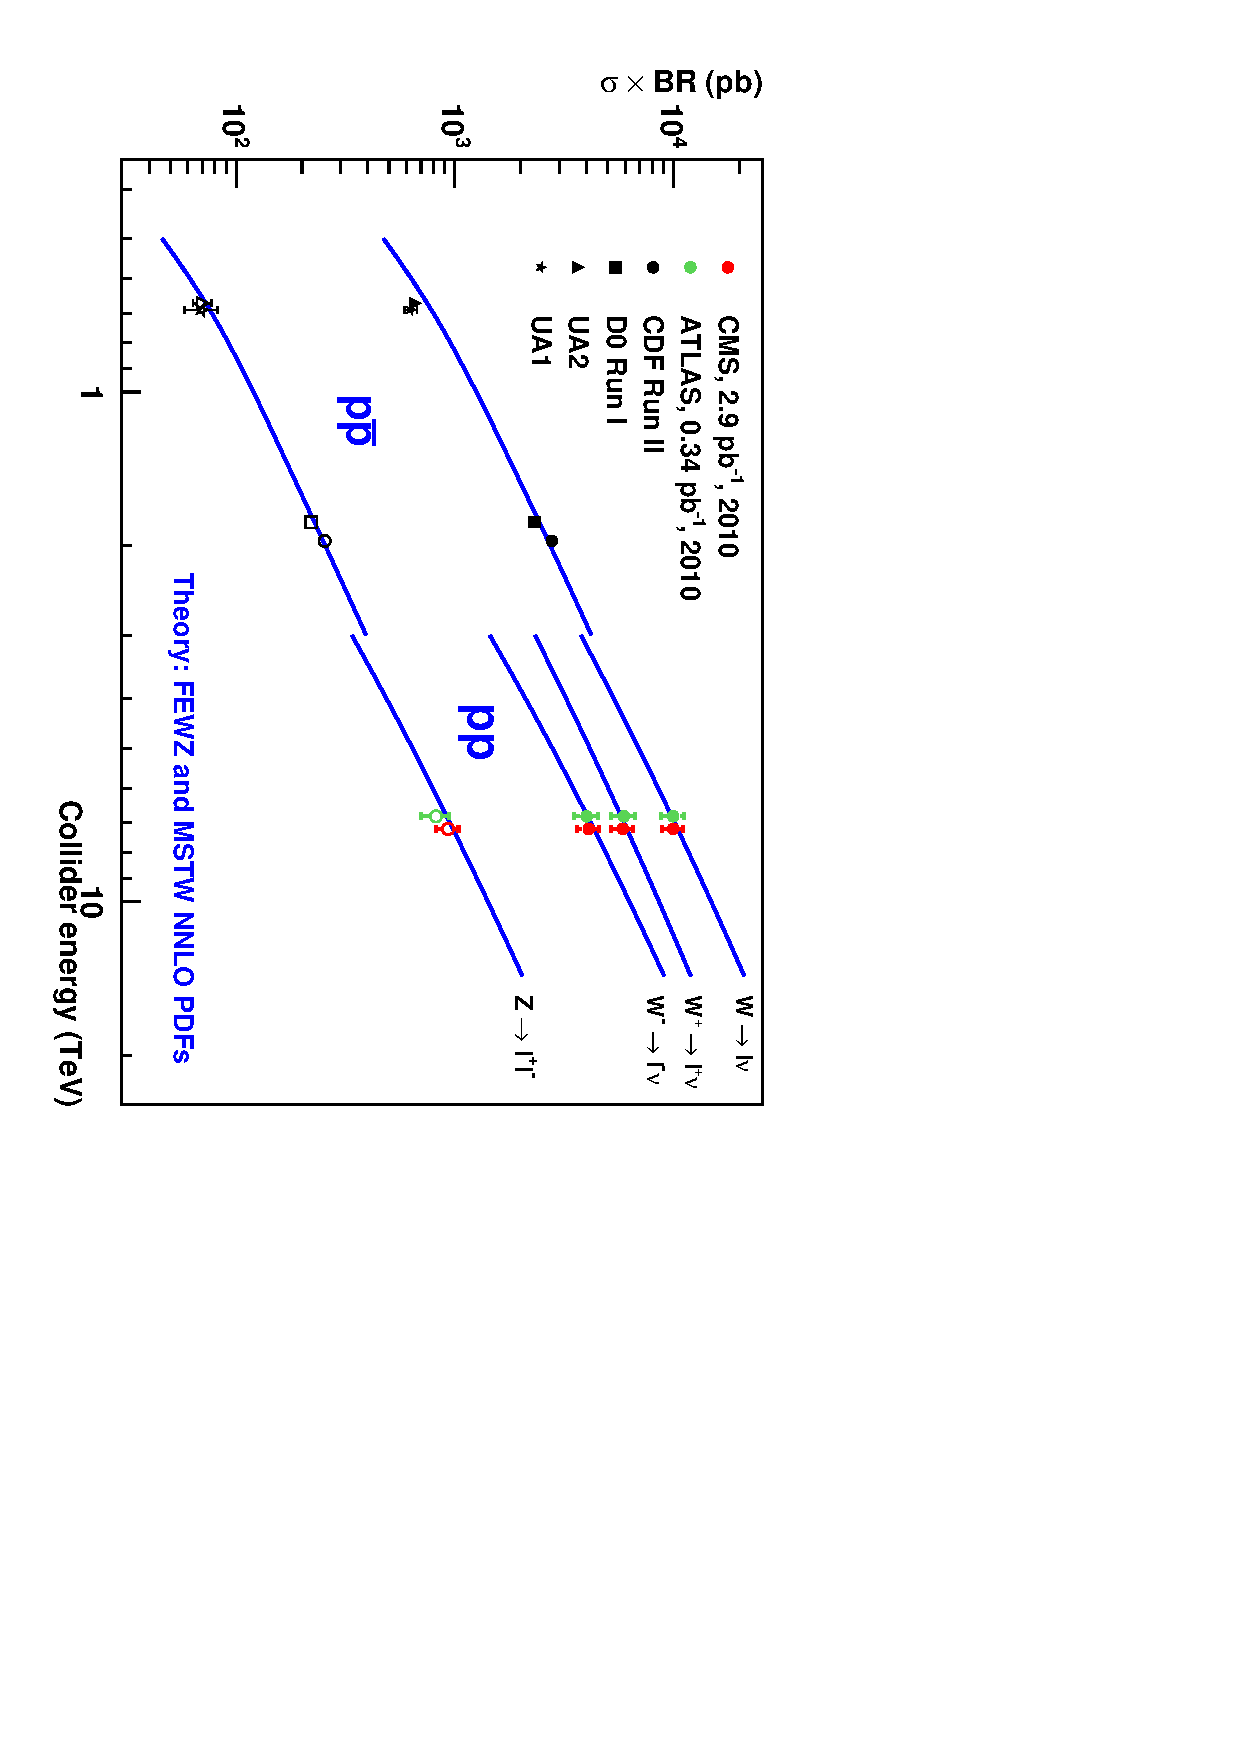
\includegraphics[width=0.49\textwidth]{figs/Results_fake.pdf}
% \\
%   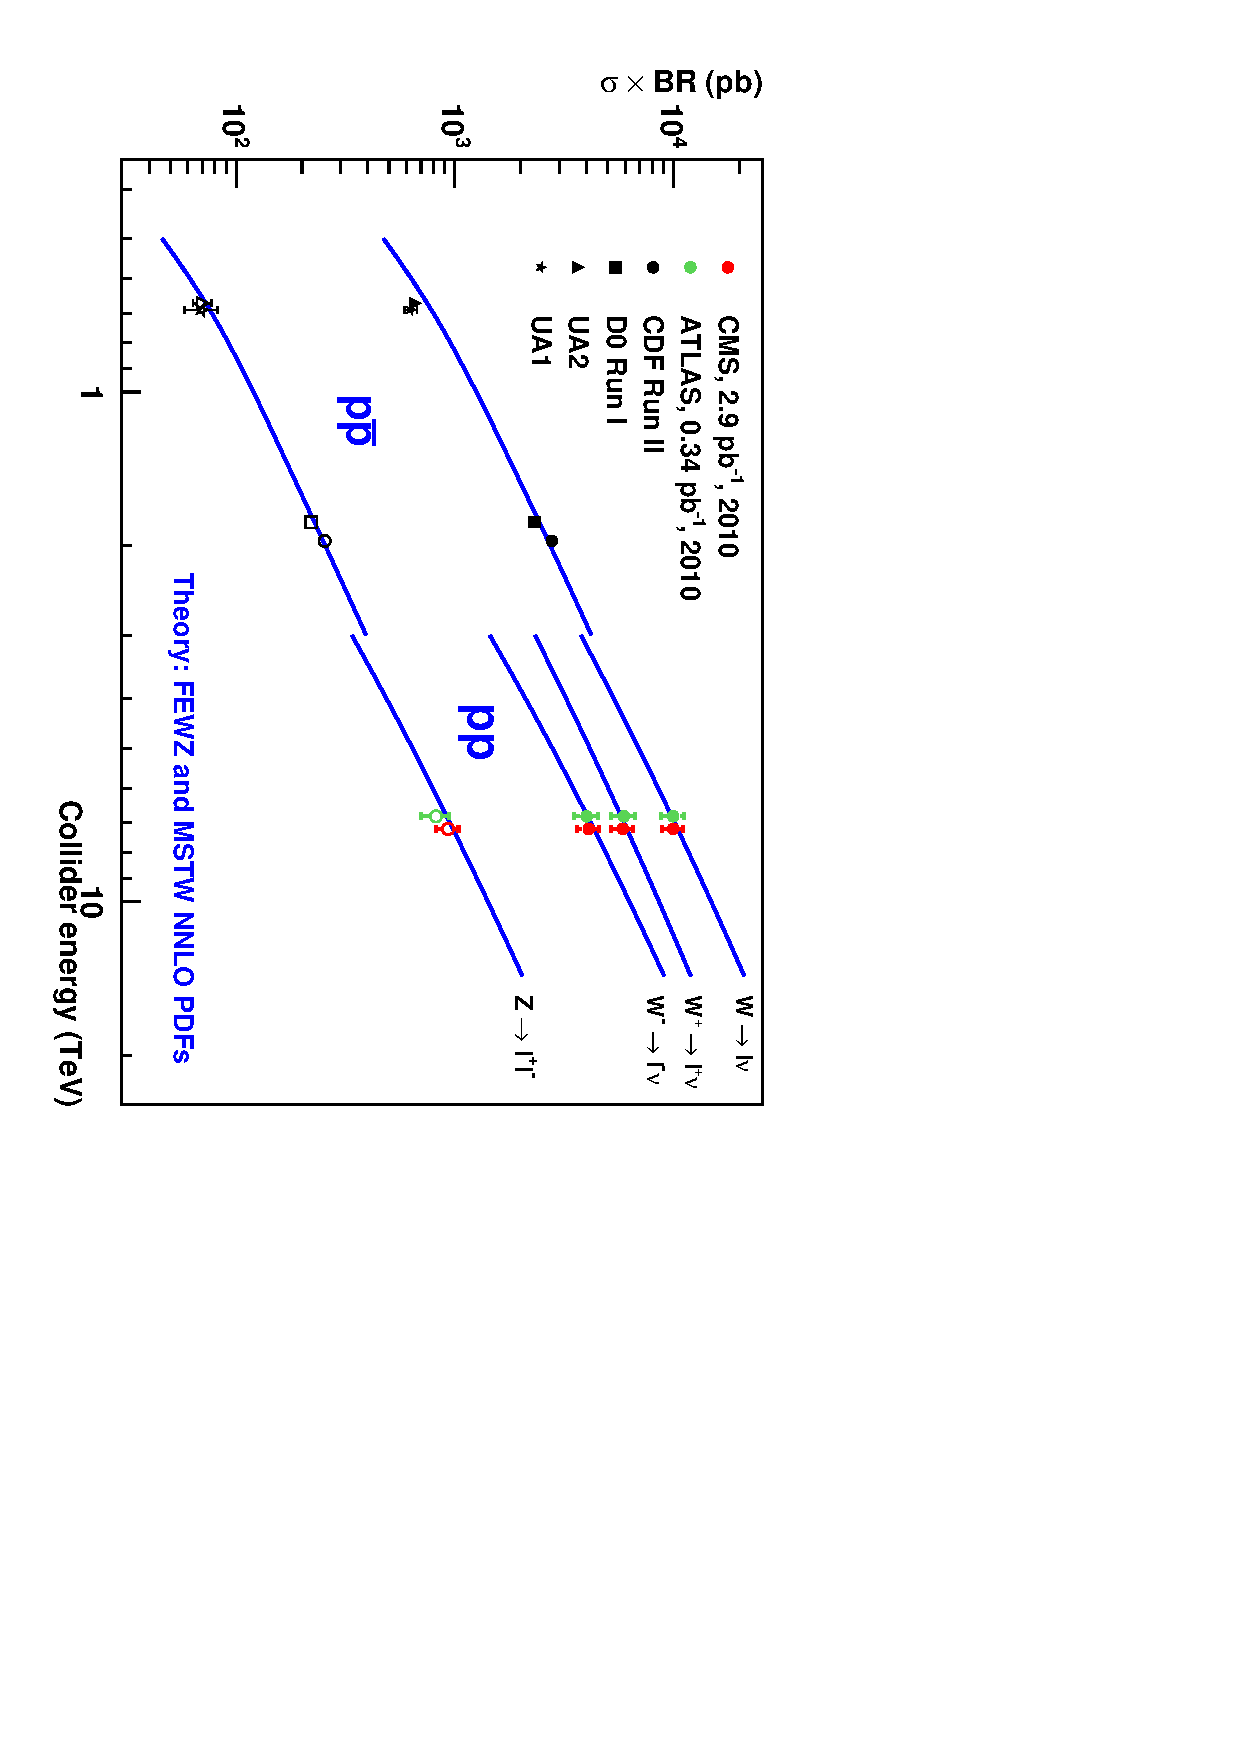
\includegraphics[width=0.49\textwidth]{figs/Results_fake.pdf}
% \caption[.]{\label{fig:Compare_LEPstylePlots}
% Comparaison of the present CMS measurements ($2.9~\invpb$) 
% with CMS preliminary measurements
% for ICHEP ($198~\invnb$) and with ATLAS submitted measurements 
% ($320~\invnb$). }
% \end{center}
% \end{figure}

\begin{figure}
\begin{center}
  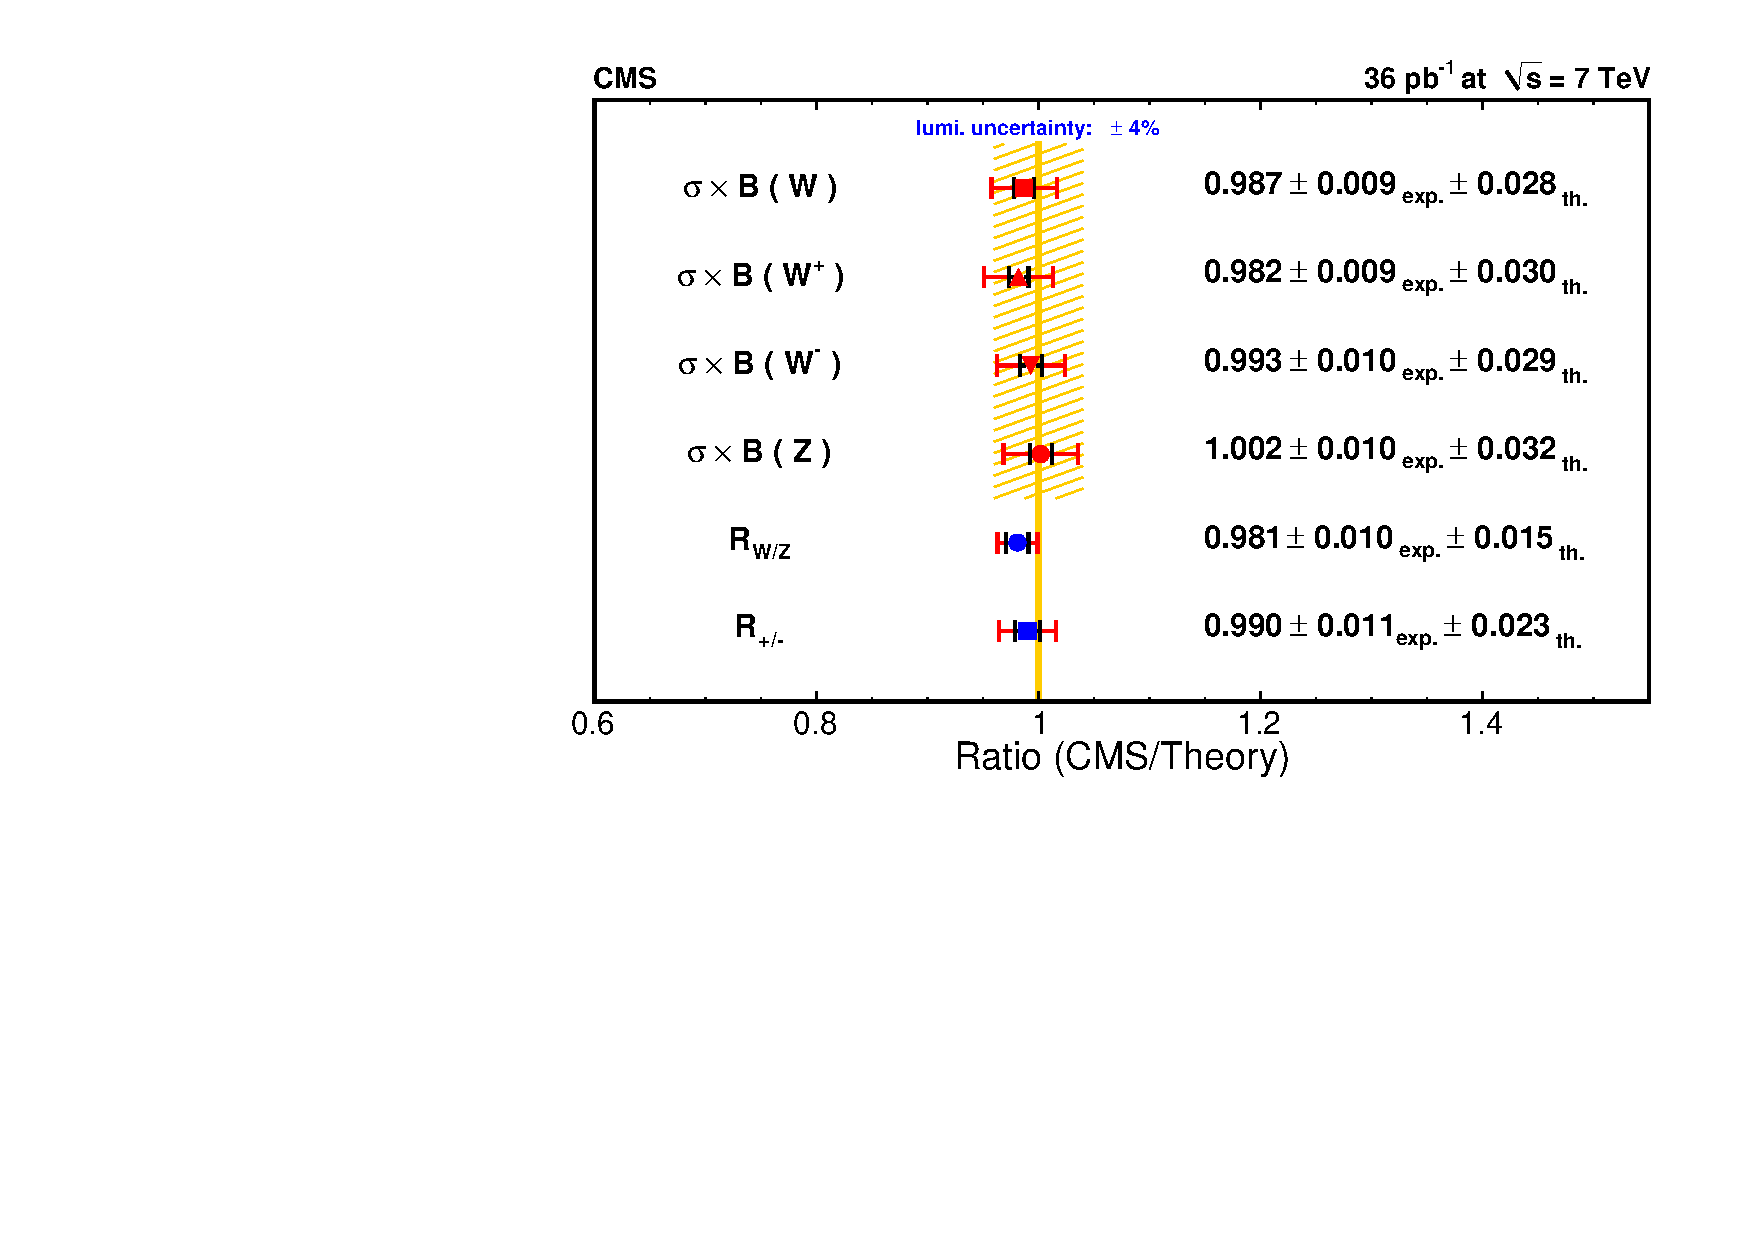
\includegraphics[width=0.9\textwidth]{figs/Results_ratioTheory.pdf}
\caption[.]{\label{fig:RatioCMSTHY}
Summary of ratios of CMS measurements to the theoretical values. }
\end{center}
\end{figure}

\begin{figure}
\begin{center}
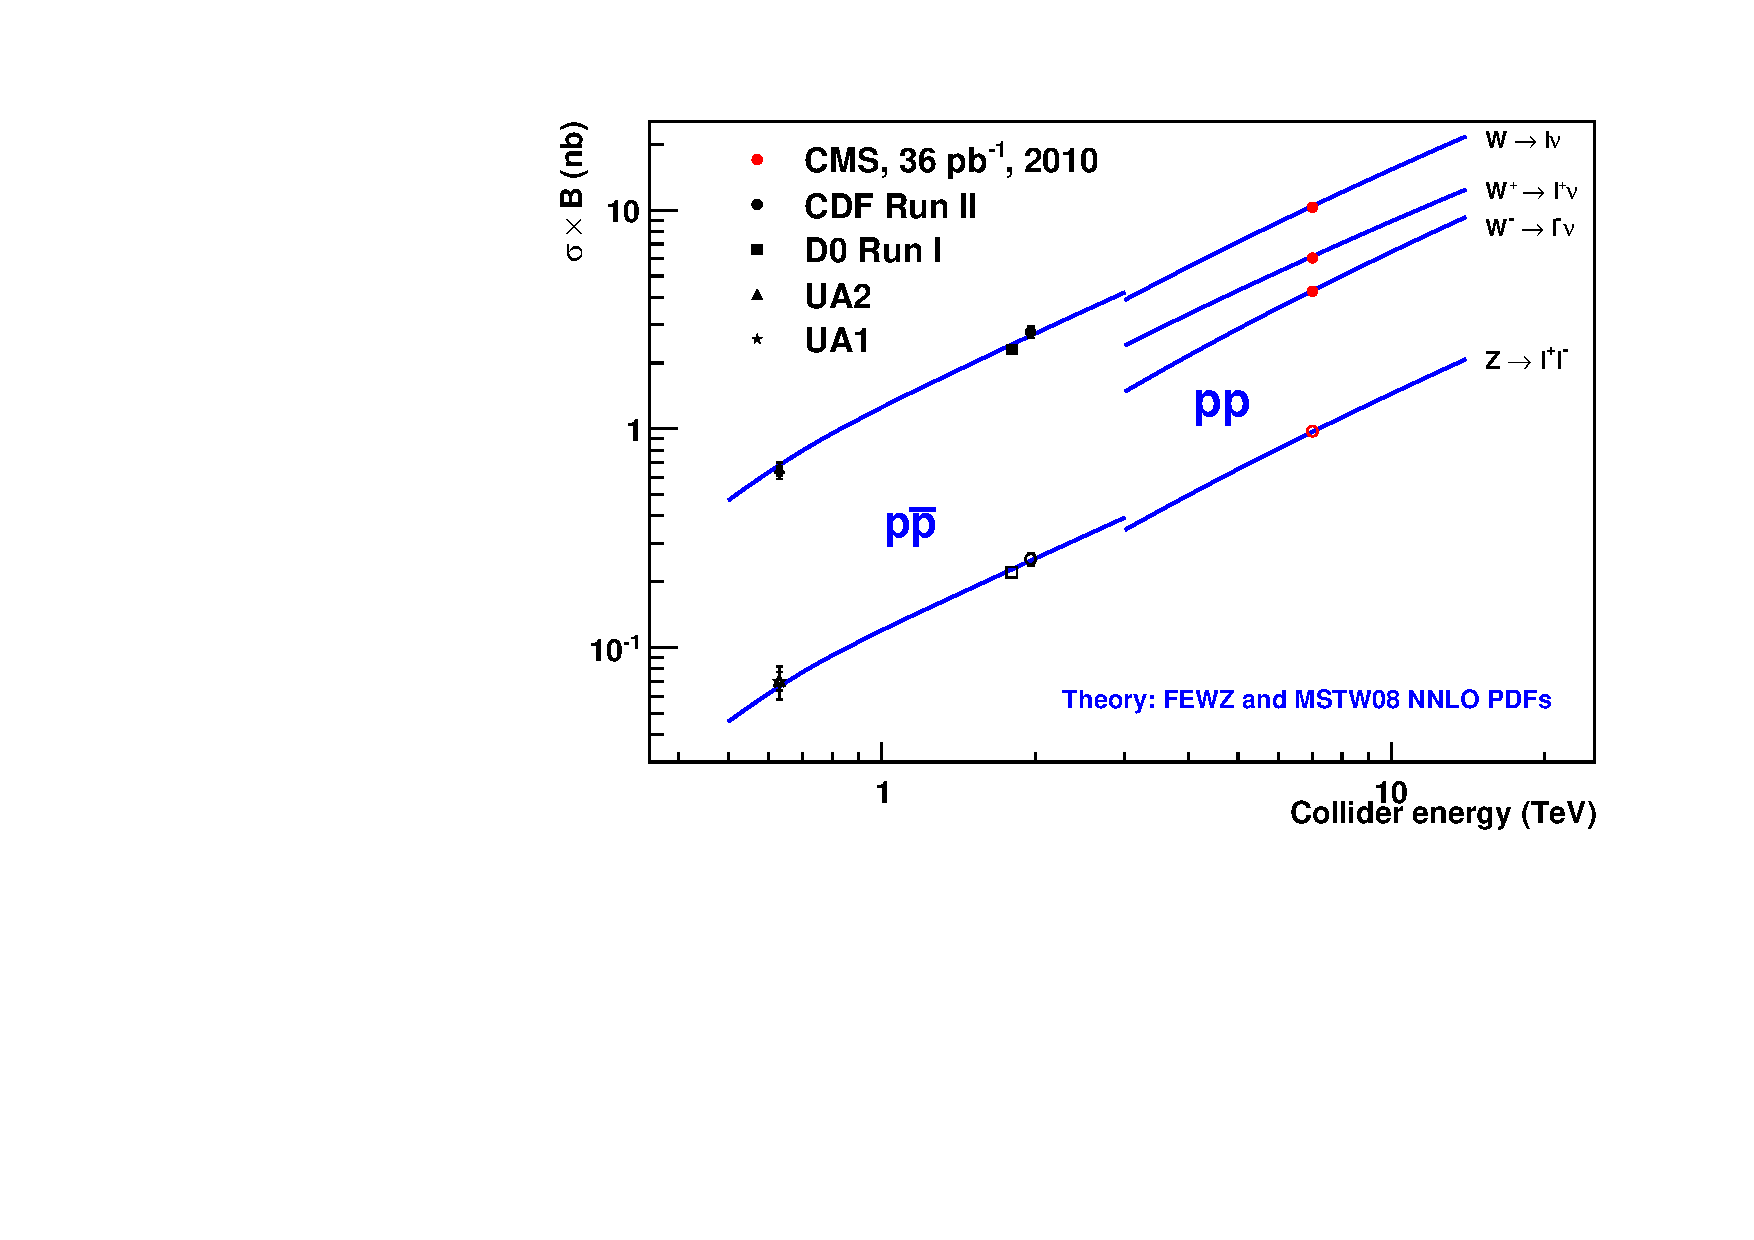
\includegraphics[width=0.9\textwidth]{figs/WZsigmas.pdf}
\caption[.]{\label{fig:WZsigmas}
Measurements of inclusive cross sections from CMS and experiments
at lower-energy colliders.  The solid symbols represent
$\sigma( \pp \to \Wo X)\times BF(\Wo\rightarrow\ell\nu)$ and the
hollow symbols, $\sigma(\pp\to\Zo X)\times BF(\Zo\rightarrow\ell^+\ell^-)$.}
\end{center}
\end{figure}


\begin{table} %
\begin{center}
\caption[.]{ Summary of ratios of CMS measurements to the theoretical values. }
\begin{tabular}{|l|c|}
\hline
Quantity & Ratio (CMS/Theory) \\
\hline
$\SIGBRSHORT{\Wpm}$   & $\RATCMSTHYWI$ \\
$\SIGBRSHORT{\Wp}$     & $\RATCMSTHYWP$ \\
$\SIGBRSHORT{\Wm}$     & $\RATCMSTHYWM$ \\
$\SIGBRSHORT{\Zo}$       & $\RATCMSTHYZ$  \\
$\SIGBRSHORT{\Wo}/\SIGBRSHORT{\Zo}$     & $\RATCMSTHYWZ$ \\
$\SIGBRSHORT{\Wp}/\SIGBRSHORT{\Wm}$ & $\RATCMSTHYWW$ \\
\hline
\end{tabular}
\label{tab:RatioCMSTHY}
\end{center}
\end{table}

